\begin{figure}[th!]
    \centering
    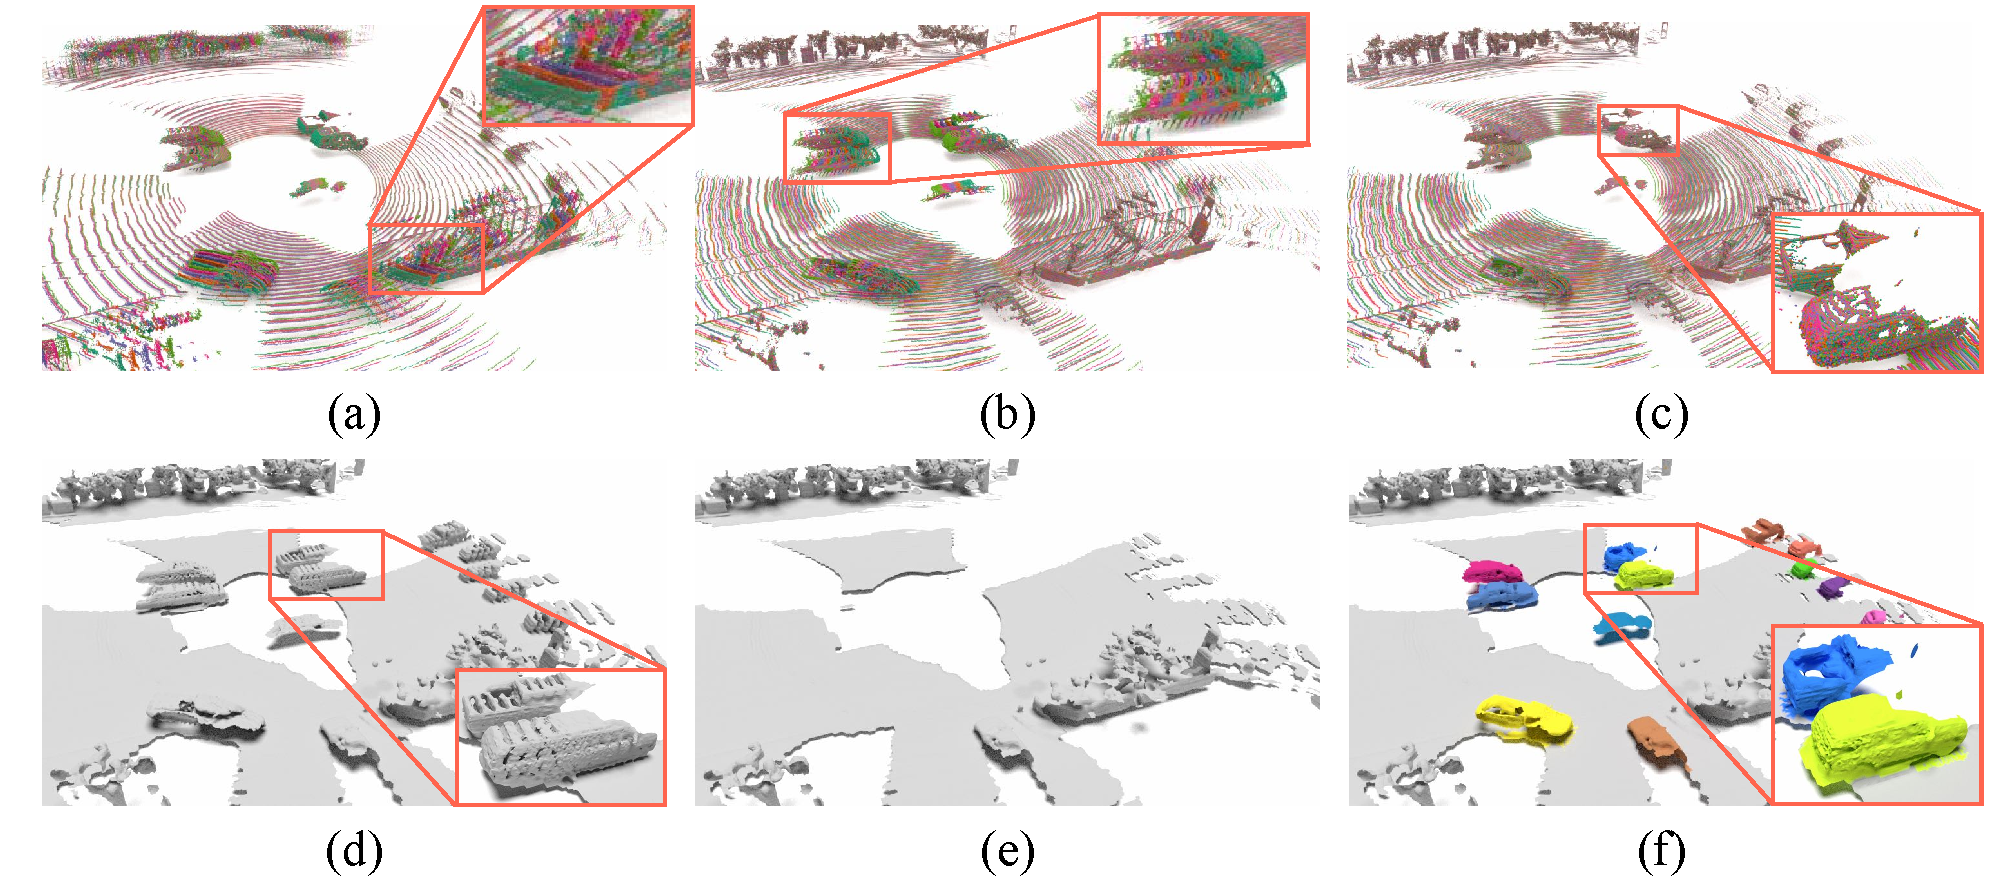
\includegraphics[width=\columnwidth]{figs/figure/teaser.pdf}
    \caption{Points in LiDAR frames acquired over time are not aligned due to the motion of the sensor and of other agents in the scene (a, d). Static background points can be aligned using ego-motion, but this smears the dynamic points across their trajectories (b). While motion segmentation only enables removing the moving points from the scene (e), our method properly disentangles individual moving objects from the static part and accumulates both correctly (c, f).}
   \label{fig:teaser}
\end{figure}